\mbox{}


\chapter{Entrenamiento del modelo mediante Google Colab}
\label{ch:chapter2}
Dentro del entrenamiento de modelos Deep Learning~\cite{advanced_convolutional_network} la velocidad es uno de los parámetros fundamentales.
Los modelos pueden requerir entradas de tamaño masivo en las que la capacidad de cómputo se torne clave para acelerar el proceso;
esto permite enfocarse plenamente en la mejora de rendimiento del modelo planteado.
El objetivo es evitar la posible espera que pueda producir volver a entrenar el modelo con distintos parámetros.
Con ello, se puede reajustar constantemente para encontrar el punto óptimo de manera ágil.

En este trabajo se va a entrenar un modelo de \texit{Deep Learning} haciendo uso del framework de código abierto de TensorFlow\footnote{\url{https://www.tensorflow.org/}}, que está programado en el lenguaje de programación Python.
Éste incluye una API (Interfaz de Programación de Aplicaciones) de Deep Learning llamada Keras, que será la que utilicemos.

El tipo de operaciones que requiere nuestra aplicación en la parte del tratamiento de imágenes, así como los procedimientos que realizan las redes neuronales~\cite{neural_network} para hacer sus cálculos son, en muchas ocasiones, operaciones matriciales. Nuestro objetivo será aprovechar al máximo el rendimiento que una GPU (Unidad de Procesamiento Gráfico) puede aportar en este tipo de operaciones, principalmente por su arquitectura de paralelización, idónea para este tipo de trabajo.
La ventaja que aporta frente a la CPU (Unidad de Procesamiento Central) es la capacidad de cómputo con un mayor número de núcleos o cores (ver Figura~\ref{fig:Arquitectura de paralelización de una GPU}), gracias a su conectividad por PCI express y el ancho de banda que proporciona.

Cabe mencionar que Google Colab, al ser una plataforma gratuita, no asegura la disponibilidad de sus componentes.
Esto conlleva que tanto el hardware requerido como su memoria disponible pueda variar según la demanda del sistema.
En este trabajo se han mantenido los mismos componentes hardware en Google Colab con la máxima memoria disponible.
\begin{figure}[h]
    \centering
    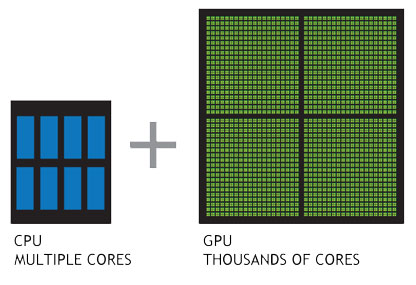
\includegraphics[width=0.5\textwidth]{images/chapter2/cpu-and-gpu.jpg}
    %\caption{Arquitectura de paralelización de una GPU.}
    \caption{Diferencia de núcleos para procesar cargas de trabajo en paralelo de forma eficiente entre CPU y GPU.}
    \label{fig:Arquitectura de paralelización de una GPU}
\end{figure}


\section{Modelo propuesto}\label{sec:modelo-propuesto}
En esta parte del trabajo se pretende conseguir la máxima velocidad de entrenamiento posible manteniendo unos niveles de acierto elevados en la predicción.

Nuestro modelo \cite{paper_project} tiene como cometido primordial poder clasificar distintas imágenes según el estado del terreno que aparece en la fotografía, siendo las opciones: terreno dañado y terreno en buenas condiciones. Para ello, disponemos de un dataset de 268 imágenes multiespectrales, adquirido por el satélite de observación terrestre de alta resolución GeoEye-1 durante el terremoto ocurrido en Haití en 2010. En este tipo de imágenes se capturan datos dentro de rangos de longitud de onda específicos a través del espectro electromagnético visible. En la Figura \ref{fig:terrain} podemos observer un ejemplo del tipo de imágenes que se usarán en este trabajo.



Como framework principal para realizar el entrenamiento nos ayudaremos de TensorFlow, que incluye la librería de \texit{Deep Learning} Keras. Esta librería simplifica mucho la implementación de este tipo de algoritmos de aprendizaje automático, debido a que sus objetos y funciones están programados de una manera intuitiva.

La distribución a efectuar sobre el conjunto de datos en entrenamiento y test es del 70\% y 30\% respectivamente.

\begin{figure}[h]
\centering
    \begin{tabular}{cc}
        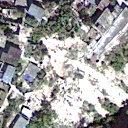
\includegraphics[height=0.35\textwidth]{images/chapter2/post_114_019.png} &
        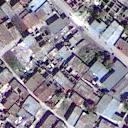
\includegraphics[height=0.35\textwidth]{images/chapter2/post_001_079.png}\\
        (a) & (b)\\
    \end{tabular}
    \caption{Ejemplo de imagen capturada por el satélite GeoEye-1. (a) Imagen de un terreno destruido. (b) Imagen de un terreno en buenas condiciones.}    \label{fig:terrain}
\end{figure}
Para la construcción de este modelo haremos uso de las siguientes capas, sobre las que TensorFlow nos da una API para tener control total sobre su configuración. Son descritas a continuación:

\begin{itemize}
    \item \textbf{Conv2D}: capa convolucional cuyo principal objetivo es extraer características de la imagen de entrada o/y sus partes.
    El término 2D se refiere al movimiento del filtro, un parámetro de entrada de este tipo de capas.
    El filtro atraviesa la imagen en dos dimensiones.
    Tiene como parámetros de entrada una imagen en tres dimensiones y el número de filtros que vamos a aplicar sobre la imagen.

    Aplicaremos sobre esta capa una configuración de 64 filtros y un tamaño de kernel de 3$\times$3 ya que nuestras imágenes son de 128$\times$128 píxeles.

    \item \textbf{Activación Relu (Recitified Linear Unit)}: en redes neuronales, una función de activación es la responsable de transformar la entrada.
    Sus principales funciones son detectar posibles correlaciones entre dos variables distintas y ayudar al modelo a tener en cuenta funciones no lineales. Ello significa que la red neuronal es capaz de realizar microajustes para capturar relaciones entre entradas y salidas que no sigan una línea recta en el plano cartesiano.

    Como podemos observar en la Figura~\ref{fig:Función de activación Relu}, la función de activación Relu se comporta devolviendo un 0 para valores de entrada negativos y, en caso contrario, devolviendo el propio valor de entrada.
    Esta función de activación conserva los valores que contienen algún patrón en la imagen y los transfiere a la siguiente capa, mientras que los pesos negativos no son importantes y son establecidos con el valor 0.
    Otras funciones de activación como la función Sigmoide o Tanh modifican todos los valores de entrada, mientras que la función Relu mantendrá los valores de peso positivo para las capas posteriores.

    \item \textbf{MaxPooling2D}: es una capa que sigue un proceso de discretización basado en muestras, y su objetivo es reducir la muestra de una representación de entrada mediante el acortamiento de sus dimensiones.
    En nuestro modelo aplicaremos una reducción a matrices de 2$\times$2.

    \begin{figure}
        \centering
        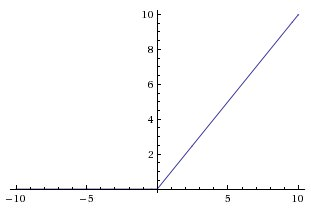
\includegraphics[width=0.5\textwidth]{images/chapter2/relu.jpg}
        \caption{Función de activación Relu.}
        \label{fig:Función de activación Relu}
    \end{figure}

    \item \textbf{Dropout}: El cometido de esta capa es ignorar ciertas neuronas de forma aleatoria para no incluirlas en el entrenamiento. Las neuronas restantes serán las encargadas de representar las predicciones de la red.
    De esta manera también reducimos la complejidad de nuestra red y la posibilidad de sobreentrenamiento.

    \item \textbf{Flatten}: capa de aplanamiento usada para reducir a uno el número de dimensiones de nuestra matriz de entrada.

    \item \textbf{Dense}: una de las capas más utilizadas en la API de Keras, es la manera de efectuar multiplicaciones matriciales.

    \item \textbf{Optimizador Adam}: es un algoritmo de optimización diseñado especialmente para redes neuronales. Aprovecha el poder de los métodos de tasas de aprendizaje adaptativo para encontrar nivel de aprendizaje individuales para cada parámetro.
    Este optimizador posee un hiperparámetro llamado \textit{learning rate} que regula la rapidez con la que el modelo avanza hacia el valor óptimo de sus pesos.
    Un \textit{learning rate} bajo implicaría que los pesos evolucionan lentamente durante el entrenamiento, con lo cual puede tardar mucho en llegar al valor óptimo, mientras que con un learning rate alto avanzamos más rápido pero podemos sobrepasar
    este punto óptimo. El valor de este hiperparámetro en este trabajo se mantiene a 0.0008.

\end{itemize}

Para un mejor entendimiento, en la Figura~\ref{fig:Topología de la red del modelo de redes neuronales.} podemos observar el conjunto de capas utilizado para crear la topología de la red de nuestro modelo. Además, algunas optimizaciones a nivel de hardware han sido realizadas para acelerar el proceso de forma general. Estas modificaciones son las siguientes:


\begin{itemize}
    \item \textbf{Uso de variables de 16 bits en vez de 32 bits}: una de las posibilidades que nos brinda el uso de una GPU es reducir a la mitad el uso en memoria de las variables del proceso.
    Usaremos esto siempre y cuando no afecte a la calidad de la predicción.
    \item \textbf{Uso del compilador XLA}: el compilador XLA\footnote{\url{https://www.tensorflow.org/xla}} (Accelerated Linear Algebra) optimiza el grafo de nuestro modelo de manera específica haciendo uso de la GPU.
    Normalmente cuando se ejecuta un programa de TensorFlow cada operación tiene una implementación de kernel de GPU previamente compilada a la que el ejecutor envía datos.
    Con el compilador XLA conseguimos fusionar en una sola ejecución todas estas operaciones, consiguiendo así reducir el ancho de banda usado en memoria.
    \item \textbf{Valores altos del parámetro de entrenamiento Batch Size}: este parámetro define el número de muestras con las que se va a ir entrenando la red hasta completar el número de registros totales. Gracias a la capacidad de cómputo de nuestra GPU podemos permitirnos el uso de valores altos en este parámetro de entrenamiento. El uso de valores pequeños puede reducir el uso de memoria y la velocidad de entrenamiento. En nuestra red el número total de registros es tan pequeño que nos permitiremos usar un valor cercano al total de imágenes que disponemos.
\end{itemize}

\begin{figure}[h]
    \centering
    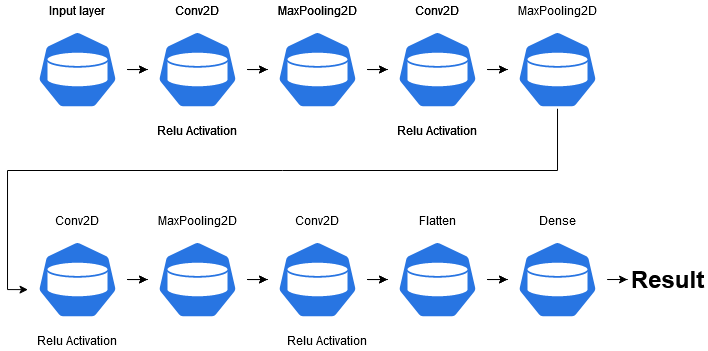
\includegraphics[width=1\textwidth]{images/chapter2/neural_network.png}
    \caption{Topología de la red del modelo \texit{Deep Learning} usado para la clasificación de daños.}
    \label{fig:Topología de la red del modelo de redes neuronales.}
\end{figure}

\section{Entorno Google Colab}\label{sec:entorno-Google-colab}
La plataforma de Google Colab\footnote{\url{https://colab.research.Google.com/notebooks/intro.ipynb}} es un servicio gratuito de Google, con el que podemos ejecutar e instalar librerías del lenguaje de programación Python~\cite{python_object_oriented}.

Una de las grandes ventajas de trabajar con este entorno es que no necesitamos configuración ninguna, se ejecuta de forma íntegra en el navegador sin necesidad de instalar nada previamente. Esto supone que toda la carga computacional reside en la herramienta de Google, lo que permite trabajar de manera fluida realizando otro tipo de actividades en nuestra máquina, o simplemente ejecutar un proceso para el que no tenemos suficiente potencia disponible.


Estas características permiten a Google Colab convertirse en un entorno muy válido para personas que están dando sus primeros pasos en este área de la inteligencia artificial, pero haciendo uso
de unas herramientas profesionales.
En este trabajo haremos uso de la GPU Tesla K80\footnote{\url{https://www.nvidia.com/es-es/data-center/tesla-k80/}}.
Las características principales de nuestra principal unidad de cómputo son las siguientes:
\begin{itemize}
    \item 4992 núcleos de NVIDIA CUDA con diseño de dos GPU\@.
    \item Hasta 2.91 teraflops de rendimiento en operaciones de precisión doble con NVIDIA GPU Boost.
    \item 24 GB de memoria GDDR5.
    \item 480 GB/s de ancho de banda de memoria agregado.
    \item Hasta 8.73 teraflops de rendimiento en operaciones de precisión simple con NVIDIA GPU Boost.
\end{itemize}

El uso de este tipo de herramientas en esta plataforma es extrapolable a otras nubes sin las restricciones en cuanto al número de unidades de procesamiento que necesitamos, la interoperabilidad de sus elementos con otros componentes externos, tales como servidores o respositorios de código, así como la configuración explícita de cada uno de los entornos de ejecución.
